% Created by tikzDevice version 0.6.2-92-0ad2792 on 2013-03-11 01:35:55
% !TEX encoding = UTF-8 Unicode
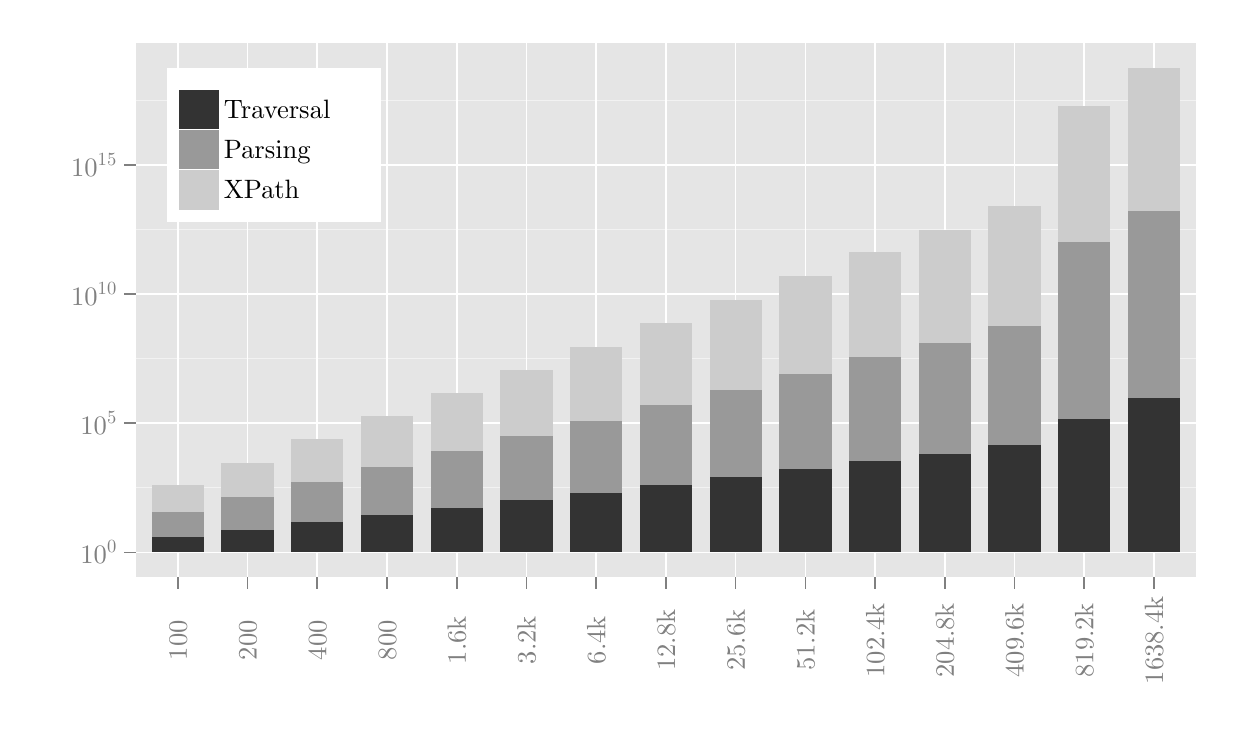
\begin{tikzpicture}[x=1pt,y=1pt]
\definecolor[named]{fillColor}{rgb}{1.00,1.00,1.00}
\path[use as bounding box,fill=fillColor,fill opacity=0.00] (0,0) rectangle (426.39,252.94);
\begin{scope}
\path[clip] (  0.00,  0.00) rectangle (426.39,252.94);
\definecolor[named]{drawColor}{rgb}{1.00,1.00,1.00}
\definecolor[named]{fillColor}{rgb}{1.00,1.00,1.00}

\path[draw=drawColor,line width= 0.6pt,line join=round,line cap=round,fill=fillColor] (  0.00, -0.00) rectangle (426.39,252.95);
\end{scope}
\begin{scope}
\path[clip] ( 39.14, 54.55) rectangle (422.13,247.25);
\definecolor[named]{fillColor}{rgb}{0.90,0.90,0.90}

\path[fill=fillColor] ( 39.14, 54.55) rectangle (422.13,247.25);
\definecolor[named]{drawColor}{rgb}{0.95,0.95,0.95}

\path[draw=drawColor,line width= 0.3pt,line join=round] ( 39.14, 86.64) --
	(422.13, 86.64);

\path[draw=drawColor,line width= 0.3pt,line join=round] ( 39.14,133.31) --
	(422.13,133.31);

\path[draw=drawColor,line width= 0.3pt,line join=round] ( 39.14,179.97) --
	(422.13,179.97);

\path[draw=drawColor,line width= 0.3pt,line join=round] ( 39.14,226.64) --
	(422.13,226.64);
\definecolor[named]{drawColor}{rgb}{1.00,1.00,1.00}

\path[draw=drawColor,line width= 0.6pt,line join=round] ( 39.14, 63.31) --
	(422.13, 63.31);

\path[draw=drawColor,line width= 0.6pt,line join=round] ( 39.14,109.97) --
	(422.13,109.97);

\path[draw=drawColor,line width= 0.6pt,line join=round] ( 39.14,156.64) --
	(422.13,156.64);

\path[draw=drawColor,line width= 0.6pt,line join=round] ( 39.14,203.31) --
	(422.13,203.31);

\path[draw=drawColor,line width= 0.6pt,line join=round] ( 54.26, 54.55) --
	( 54.26,247.25);

\path[draw=drawColor,line width= 0.6pt,line join=round] ( 79.45, 54.55) --
	( 79.45,247.25);

\path[draw=drawColor,line width= 0.6pt,line join=round] (104.65, 54.55) --
	(104.65,247.25);

\path[draw=drawColor,line width= 0.6pt,line join=round] (129.85, 54.55) --
	(129.85,247.25);

\path[draw=drawColor,line width= 0.6pt,line join=round] (155.04, 54.55) --
	(155.04,247.25);

\path[draw=drawColor,line width= 0.6pt,line join=round] (180.24, 54.55) --
	(180.24,247.25);

\path[draw=drawColor,line width= 0.6pt,line join=round] (205.44, 54.55) --
	(205.44,247.25);

\path[draw=drawColor,line width= 0.6pt,line join=round] (230.63, 54.55) --
	(230.63,247.25);

\path[draw=drawColor,line width= 0.6pt,line join=round] (255.83, 54.55) --
	(255.83,247.25);

\path[draw=drawColor,line width= 0.6pt,line join=round] (281.02, 54.55) --
	(281.02,247.25);

\path[draw=drawColor,line width= 0.6pt,line join=round] (306.22, 54.55) --
	(306.22,247.25);

\path[draw=drawColor,line width= 0.6pt,line join=round] (331.42, 54.55) --
	(331.42,247.25);

\path[draw=drawColor,line width= 0.6pt,line join=round] (356.61, 54.55) --
	(356.61,247.25);

\path[draw=drawColor,line width= 0.6pt,line join=round] (381.81, 54.55) --
	(381.81,247.25);

\path[draw=drawColor,line width= 0.6pt,line join=round] (407.01, 54.55) --
	(407.01,247.25);
\definecolor[named]{fillColor}{rgb}{0.20,0.20,0.20}

\path[fill=fillColor] ( 44.81, 63.31) rectangle ( 63.71, 68.91);
\definecolor[named]{fillColor}{rgb}{0.60,0.60,0.60}

\path[fill=fillColor] ( 44.81, 68.91) rectangle ( 63.71, 78.03);
\definecolor[named]{fillColor}{rgb}{0.80,0.80,0.80}

\path[fill=fillColor] ( 44.81, 78.03) rectangle ( 63.71, 87.82);
\definecolor[named]{fillColor}{rgb}{0.20,0.20,0.20}

\path[fill=fillColor] ( 70.00, 63.31) rectangle ( 88.90, 71.41);
\definecolor[named]{fillColor}{rgb}{0.60,0.60,0.60}

\path[fill=fillColor] ( 70.00, 71.41) rectangle ( 88.90, 83.28);
\definecolor[named]{fillColor}{rgb}{0.80,0.80,0.80}

\path[fill=fillColor] ( 70.00, 83.28) rectangle ( 88.90, 95.77);
\definecolor[named]{fillColor}{rgb}{0.20,0.20,0.20}

\path[fill=fillColor] ( 95.20, 63.31) rectangle (114.10, 74.15);
\definecolor[named]{fillColor}{rgb}{0.60,0.60,0.60}

\path[fill=fillColor] ( 95.20, 74.15) rectangle (114.10, 88.89);
\definecolor[named]{fillColor}{rgb}{0.80,0.80,0.80}

\path[fill=fillColor] ( 95.20, 88.89) rectangle (114.10,104.31);
\definecolor[named]{fillColor}{rgb}{0.20,0.20,0.20}

\path[fill=fillColor] (120.40, 63.31) rectangle (139.29, 76.73);
\definecolor[named]{fillColor}{rgb}{0.60,0.60,0.60}

\path[fill=fillColor] (120.40, 76.73) rectangle (139.29, 94.27);
\definecolor[named]{fillColor}{rgb}{0.80,0.80,0.80}

\path[fill=fillColor] (120.40, 94.27) rectangle (139.29,112.45);
\definecolor[named]{fillColor}{rgb}{0.20,0.20,0.20}

\path[fill=fillColor] (145.59, 63.31) rectangle (164.49, 79.44);
\definecolor[named]{fillColor}{rgb}{0.60,0.60,0.60}

\path[fill=fillColor] (145.59, 79.44) rectangle (164.49, 99.81);
\definecolor[named]{fillColor}{rgb}{0.80,0.80,0.80}

\path[fill=fillColor] (145.59, 99.81) rectangle (164.49,120.89);
\definecolor[named]{fillColor}{rgb}{0.20,0.20,0.20}

\path[fill=fillColor] (170.79, 63.31) rectangle (189.69, 82.15);
\definecolor[named]{fillColor}{rgb}{0.60,0.60,0.60}

\path[fill=fillColor] (170.79, 82.15) rectangle (189.69,105.32);
\definecolor[named]{fillColor}{rgb}{0.80,0.80,0.80}

\path[fill=fillColor] (170.79,105.32) rectangle (189.69,129.18);
\definecolor[named]{fillColor}{rgb}{0.20,0.20,0.20}

\path[fill=fillColor] (195.99, 63.31) rectangle (214.88, 84.93);
\definecolor[named]{fillColor}{rgb}{0.60,0.60,0.60}

\path[fill=fillColor] (195.99, 84.93) rectangle (214.88,110.88);
\definecolor[named]{fillColor}{rgb}{0.80,0.80,0.80}

\path[fill=fillColor] (195.99,110.88) rectangle (214.88,137.55);
\definecolor[named]{fillColor}{rgb}{0.20,0.20,0.20}

\path[fill=fillColor] (221.18, 63.31) rectangle (240.08, 87.74);
\definecolor[named]{fillColor}{rgb}{0.60,0.60,0.60}

\path[fill=fillColor] (221.18, 87.74) rectangle (240.08,116.55);
\definecolor[named]{fillColor}{rgb}{0.80,0.80,0.80}

\path[fill=fillColor] (221.18,116.55) rectangle (240.08,146.08);
\definecolor[named]{fillColor}{rgb}{0.20,0.20,0.20}

\path[fill=fillColor] (246.38, 63.31) rectangle (265.28, 90.53);
\definecolor[named]{fillColor}{rgb}{0.60,0.60,0.60}

\path[fill=fillColor] (246.38, 90.53) rectangle (265.28,122.17);
\definecolor[named]{fillColor}{rgb}{0.80,0.80,0.80}

\path[fill=fillColor] (246.38,122.17) rectangle (265.28,154.47);
\definecolor[named]{fillColor}{rgb}{0.20,0.20,0.20}

\path[fill=fillColor] (271.58, 63.31) rectangle (290.47, 93.47);
\definecolor[named]{fillColor}{rgb}{0.60,0.60,0.60}

\path[fill=fillColor] (271.58, 93.47) rectangle (290.47,127.96);
\definecolor[named]{fillColor}{rgb}{0.80,0.80,0.80}

\path[fill=fillColor] (271.58,127.96) rectangle (290.47,163.10);
\definecolor[named]{fillColor}{rgb}{0.20,0.20,0.20}

\path[fill=fillColor] (296.77, 63.31) rectangle (315.67, 96.46);
\definecolor[named]{fillColor}{rgb}{0.60,0.60,0.60}

\path[fill=fillColor] (296.77, 96.46) rectangle (315.67,133.76);
\definecolor[named]{fillColor}{rgb}{0.80,0.80,0.80}

\path[fill=fillColor] (296.77,133.76) rectangle (315.67,171.70);
\definecolor[named]{fillColor}{rgb}{0.20,0.20,0.20}

\path[fill=fillColor] (321.97, 63.31) rectangle (340.87, 98.99);
\definecolor[named]{fillColor}{rgb}{0.60,0.60,0.60}

\path[fill=fillColor] (321.97, 98.99) rectangle (340.87,139.04);
\definecolor[named]{fillColor}{rgb}{0.80,0.80,0.80}

\path[fill=fillColor] (321.97,139.04) rectangle (340.87,179.77);
\definecolor[named]{fillColor}{rgb}{0.20,0.20,0.20}

\path[fill=fillColor] (347.17, 63.31) rectangle (366.06,102.07);
\definecolor[named]{fillColor}{rgb}{0.60,0.60,0.60}

\path[fill=fillColor] (347.17,102.07) rectangle (366.06,145.02);
\definecolor[named]{fillColor}{rgb}{0.80,0.80,0.80}

\path[fill=fillColor] (347.17,145.02) rectangle (366.06,188.55);
\definecolor[named]{fillColor}{rgb}{0.20,0.20,0.20}

\path[fill=fillColor] (372.36, 63.31) rectangle (391.26,111.52);
\definecolor[named]{fillColor}{rgb}{0.60,0.60,0.60}

\path[fill=fillColor] (372.36,111.52) rectangle (391.26,175.43);
\definecolor[named]{fillColor}{rgb}{0.80,0.80,0.80}

\path[fill=fillColor] (372.36,175.43) rectangle (391.26,224.47);
\definecolor[named]{fillColor}{rgb}{0.20,0.20,0.20}

\path[fill=fillColor] (397.56, 63.31) rectangle (416.46,119.25);
\definecolor[named]{fillColor}{rgb}{0.60,0.60,0.60}

\path[fill=fillColor] (397.56,119.25) rectangle (416.46,186.81);
\definecolor[named]{fillColor}{rgb}{0.80,0.80,0.80}

\path[fill=fillColor] (397.56,186.81) rectangle (416.46,238.50);
\end{scope}
\begin{scope}
\path[clip] (  0.00,  0.00) rectangle (426.39,252.94);
\definecolor[named]{drawColor}{rgb}{0.50,0.50,0.50}

\node[text=drawColor,anchor=base west,inner sep=0pt, outer sep=0pt, scale=  0.96] at ( 19.07, 59.19) {10};

\node[text=drawColor,anchor=base west,inner sep=0pt, outer sep=0pt, scale=  0.67] at ( 28.67, 63.12) {0};

\node[text=drawColor,anchor=base west,inner sep=0pt, outer sep=0pt, scale=  0.96] at ( 19.07,105.86) {10};

\node[text=drawColor,anchor=base west,inner sep=0pt, outer sep=0pt, scale=  0.67] at ( 28.67,109.78) {5};

\node[text=drawColor,anchor=base west,inner sep=0pt, outer sep=0pt, scale=  0.96] at ( 15.71,152.52) {10};

\node[text=drawColor,anchor=base west,inner sep=0pt, outer sep=0pt, scale=  0.67] at ( 25.31,156.45) {1};

\node[text=drawColor,anchor=base west,inner sep=0pt, outer sep=0pt, scale=  0.67] at ( 28.67,156.45) {0};

\node[text=drawColor,anchor=base west,inner sep=0pt, outer sep=0pt, scale=  0.96] at ( 15.71,199.19) {10};

\node[text=drawColor,anchor=base west,inner sep=0pt, outer sep=0pt, scale=  0.67] at ( 25.31,203.11) {1};

\node[text=drawColor,anchor=base west,inner sep=0pt, outer sep=0pt, scale=  0.67] at ( 28.67,203.11) {5};
\end{scope}
\begin{scope}
\path[clip] (  0.00,  0.00) rectangle (426.39,252.94);
\definecolor[named]{drawColor}{rgb}{0.50,0.50,0.50}

\path[draw=drawColor,line width= 0.6pt,line join=round] ( 34.87, 63.31) --
	( 39.14, 63.31);

\path[draw=drawColor,line width= 0.6pt,line join=round] ( 34.87,109.97) --
	( 39.14,109.97);

\path[draw=drawColor,line width= 0.6pt,line join=round] ( 34.87,156.64) --
	( 39.14,156.64);

\path[draw=drawColor,line width= 0.6pt,line join=round] ( 34.87,203.31) --
	( 39.14,203.31);
\end{scope}
\begin{scope}
\path[clip] (  0.00,  0.00) rectangle (426.39,252.94);
\definecolor[named]{drawColor}{rgb}{0.50,0.50,0.50}

\path[draw=drawColor,line width= 0.6pt,line join=round] ( 54.26, 50.28) --
	( 54.26, 54.55);

\path[draw=drawColor,line width= 0.6pt,line join=round] ( 79.45, 50.28) --
	( 79.45, 54.55);

\path[draw=drawColor,line width= 0.6pt,line join=round] (104.65, 50.28) --
	(104.65, 54.55);

\path[draw=drawColor,line width= 0.6pt,line join=round] (129.85, 50.28) --
	(129.85, 54.55);

\path[draw=drawColor,line width= 0.6pt,line join=round] (155.04, 50.28) --
	(155.04, 54.55);

\path[draw=drawColor,line width= 0.6pt,line join=round] (180.24, 50.28) --
	(180.24, 54.55);

\path[draw=drawColor,line width= 0.6pt,line join=round] (205.44, 50.28) --
	(205.44, 54.55);

\path[draw=drawColor,line width= 0.6pt,line join=round] (230.63, 50.28) --
	(230.63, 54.55);

\path[draw=drawColor,line width= 0.6pt,line join=round] (255.83, 50.28) --
	(255.83, 54.55);

\path[draw=drawColor,line width= 0.6pt,line join=round] (281.02, 50.28) --
	(281.02, 54.55);

\path[draw=drawColor,line width= 0.6pt,line join=round] (306.22, 50.28) --
	(306.22, 54.55);

\path[draw=drawColor,line width= 0.6pt,line join=round] (331.42, 50.28) --
	(331.42, 54.55);

\path[draw=drawColor,line width= 0.6pt,line join=round] (356.61, 50.28) --
	(356.61, 54.55);

\path[draw=drawColor,line width= 0.6pt,line join=round] (381.81, 50.28) --
	(381.81, 54.55);

\path[draw=drawColor,line width= 0.6pt,line join=round] (407.01, 50.28) --
	(407.01, 54.55);
\end{scope}
\begin{scope}
\path[clip] (  0.00,  0.00) rectangle (426.39,252.94);
\definecolor[named]{drawColor}{rgb}{0.50,0.50,0.50}

\node[text=drawColor,rotate= 90.00,anchor=base,inner sep=0pt, outer sep=0pt, scale=  0.96] at ( 57.56, 31.57) {100};

\node[text=drawColor,rotate= 90.00,anchor=base,inner sep=0pt, outer sep=0pt, scale=  0.96] at ( 82.76, 31.57) {200};

\node[text=drawColor,rotate= 90.00,anchor=base,inner sep=0pt, outer sep=0pt, scale=  0.96] at (107.96, 31.57) {400};

\node[text=drawColor,rotate= 90.00,anchor=base,inner sep=0pt, outer sep=0pt, scale=  0.96] at (133.15, 31.57) {800};

\node[text=drawColor,rotate= 90.00,anchor=base,inner sep=0pt, outer sep=0pt, scale=  0.96] at (158.35, 31.57) {1.6k};

\node[text=drawColor,rotate= 90.00,anchor=base,inner sep=0pt, outer sep=0pt, scale=  0.96] at (183.55, 31.57) {3.2k};

\node[text=drawColor,rotate= 90.00,anchor=base,inner sep=0pt, outer sep=0pt, scale=  0.96] at (208.74, 31.57) {6.4k};

\node[text=drawColor,rotate= 90.00,anchor=base,inner sep=0pt, outer sep=0pt, scale=  0.96] at (233.94, 31.57) {12.8k};

\node[text=drawColor,rotate= 90.00,anchor=base,inner sep=0pt, outer sep=0pt, scale=  0.96] at (259.13, 31.57) {25.6k};

\node[text=drawColor,rotate= 90.00,anchor=base,inner sep=0pt, outer sep=0pt, scale=  0.96] at (284.33, 31.57) {51.2k};

\node[text=drawColor,rotate= 90.00,anchor=base,inner sep=0pt, outer sep=0pt, scale=  0.96] at (309.53, 31.57) {102.4k};

\node[text=drawColor,rotate= 90.00,anchor=base,inner sep=0pt, outer sep=0pt, scale=  0.96] at (334.72, 31.57) {204.8k};

\node[text=drawColor,rotate= 90.00,anchor=base,inner sep=0pt, outer sep=0pt, scale=  0.96] at (359.92, 31.57) {409.6k};

\node[text=drawColor,rotate= 90.00,anchor=base,inner sep=0pt, outer sep=0pt, scale=  0.96] at (385.12, 31.57) {819.2k};

\node[text=drawColor,rotate= 90.00,anchor=base,inner sep=0pt, outer sep=0pt, scale=  0.96] at (410.31, 31.57) {1638.4k};
\end{scope}
\begin{scope}
\path[clip] (  0.00,  0.00) rectangle (426.39,252.94);
\definecolor[named]{fillColor}{rgb}{1.00,1.00,1.00}

\path[fill=fillColor] ( 50.35,182.88) rectangle (127.51,238.40);
\end{scope}
\begin{scope}
\path[clip] (  0.00,  0.00) rectangle (426.39,252.94);
\definecolor[named]{drawColor}{rgb}{1.00,1.00,1.00}
\definecolor[named]{fillColor}{rgb}{0.95,0.95,0.95}

\path[draw=drawColor,line width= 0.6pt,line join=round,line cap=round,fill=fillColor] ( 54.62,216.06) rectangle ( 69.07,230.51);
\end{scope}
\begin{scope}
\path[clip] (  0.00,  0.00) rectangle (426.39,252.94);
\definecolor[named]{fillColor}{rgb}{0.20,0.20,0.20}

\path[fill=fillColor] ( 54.62,216.06) rectangle ( 69.07,230.51);

\path[] ( 54.62,216.06) --
	( 69.07,230.51);
\end{scope}
\begin{scope}
\path[clip] (  0.00,  0.00) rectangle (426.39,252.94);
\definecolor[named]{drawColor}{rgb}{1.00,1.00,1.00}
\definecolor[named]{fillColor}{rgb}{0.95,0.95,0.95}

\path[draw=drawColor,line width= 0.6pt,line join=round,line cap=round,fill=fillColor] ( 54.62,201.61) rectangle ( 69.07,216.06);
\end{scope}
\begin{scope}
\path[clip] (  0.00,  0.00) rectangle (426.39,252.94);
\definecolor[named]{fillColor}{rgb}{0.60,0.60,0.60}

\path[fill=fillColor] ( 54.62,201.61) rectangle ( 69.07,216.06);

\path[] ( 54.62,201.61) --
	( 69.07,216.06);
\end{scope}
\begin{scope}
\path[clip] (  0.00,  0.00) rectangle (426.39,252.94);
\definecolor[named]{drawColor}{rgb}{1.00,1.00,1.00}
\definecolor[named]{fillColor}{rgb}{0.95,0.95,0.95}

\path[draw=drawColor,line width= 0.6pt,line join=round,line cap=round,fill=fillColor] ( 54.62,187.15) rectangle ( 69.07,201.61);
\end{scope}
\begin{scope}
\path[clip] (  0.00,  0.00) rectangle (426.39,252.94);
\definecolor[named]{fillColor}{rgb}{0.80,0.80,0.80}

\path[fill=fillColor] ( 54.62,187.15) rectangle ( 69.07,201.61);

\path[] ( 54.62,187.15) --
	( 69.07,201.61);
\end{scope}
\begin{scope}
\path[clip] (  0.00,  0.00) rectangle (426.39,252.94);
\definecolor[named]{drawColor}{rgb}{0.00,0.00,0.00}

\node[text=drawColor,anchor=base west,inner sep=0pt, outer sep=0pt, scale=  0.96] at ( 70.88,219.98) {Traversal $\;\;\;\;$};
\end{scope}
\begin{scope}
\path[clip] (  0.00,  0.00) rectangle (426.39,252.94);
\definecolor[named]{drawColor}{rgb}{0.00,0.00,0.00}

\node[text=drawColor,anchor=base west,inner sep=0pt, outer sep=0pt, scale=  0.96] at ( 70.88,205.53) {Parsing $\;\;\;\;$};
\end{scope}
\begin{scope}
\path[clip] (  0.00,  0.00) rectangle (426.39,252.94);
\definecolor[named]{drawColor}{rgb}{0.00,0.00,0.00}

\node[text=drawColor,anchor=base west,inner sep=0pt, outer sep=0pt, scale=  0.96] at ( 70.88,191.07) {XPath $\;\;\;\;$};
\end{scope}
\end{tikzpicture}
